The crab drive layer is a vital layer to this project. It's major function shall be to make Smart Cart mobile. It comprises comprises such vital elements as the micro-controller, the motor-controllers and the drive system interface.
\subsection{MOTOR CONTROL SUBSYSTEM}
The motor control subsystem will contain a roller chain that will be responsible for steering the the cart and maintain a consistent orientation for all the wheels, a central motor to coordinate the movement of the four wheels and wheel motors to drive the wheels
\begin{figure}[h!]
	\centering
 	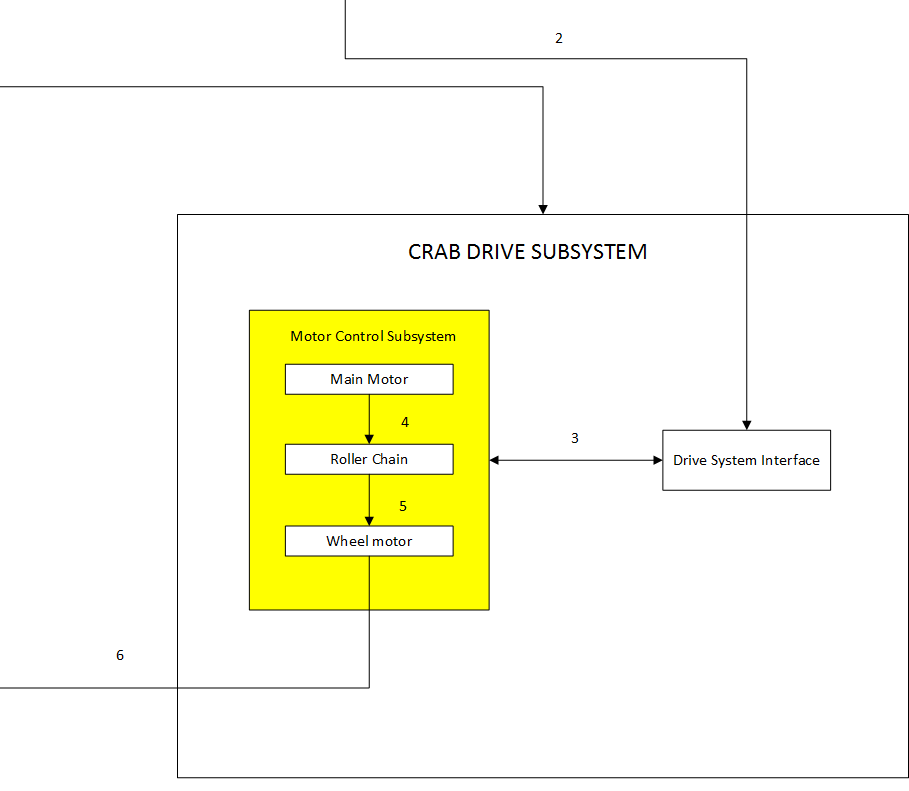
\includegraphics[width=0.60\textwidth]{images/motorcontrol}
 \caption{Motor Control subsystem description diagram}
\end{figure}

\subsection{ASSUMPTIONS}
Assumptions made are as follows:
\begin{itemize}
\item The main motor will correctly steer the wheels with the roller chain
\item The main motor will have a method to accurately keep wheel orientation data
\item The wheel motors will move the wheels accordingly
\end{itemize}

\subsection{RESPONSIBILITIES}
The main motor subsystem's responsibilities are as follows:
\begin{itemize}
\item Receive steering instructions from the drive system interface and accurately perform instructions.
\end{itemize}

\subsection{SUBSYSTEM INTERFACES}
\begin{table}[H]
\caption{Motor Control subsystem interface}
\begin{center}
\begin{tabular}{ | p{1cm} | p{6cm} | p{4cm} | p{4cm} |}
    \hline
    ID & Description & Inputs & Outputs \\ \hline
    \ 3 & Feedback data & \pbox{3cm}{N/A} & \pbox{4cm}{Drive system interface}  \\ \hline
    \ 6 & Steer Wheels & \pbox{3cm}{Drive system interface} & \pbox{4cm}{Wheel motors}  \\ \hline
\end{tabular}
\end{center}
\end{table}


\subsection{DRIVE SYSTEM INTERFACE SUBSYSTEM}
The drive system interface s designed to communicate with the navigation subsystem's camera interface it will get navigation data from the camera interface to steer the main drive motor as well as receiving feedback information for the wheel orientations.

\begin{figure}[h!]
	\centering
 	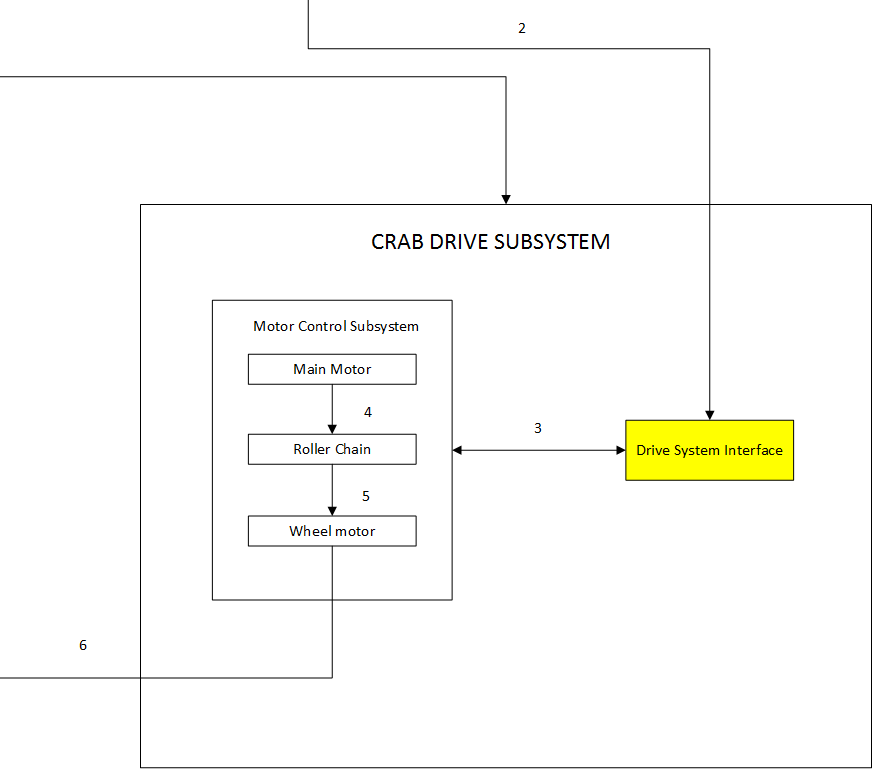
\includegraphics[width=0.60\textwidth]{images/drivesysteminterface}
 \caption{Drive system interface subsystem description diagram}
\end{figure}

\subsection{ASSUMPTIONS}
Assumptions made are as follows:
\begin{itemize}
\item The drive system interface will receive accurate navigation data from the camera interface.
\item The drive system will receive accurate feedback from the motor control subsystem.
\item The drive system interface will receive accurate feedback data from the main motor about wheel orientation
\end{itemize}

\subsubsection{RESPONSIBILITIES}
The responsibilites for drive system interface are as follows:
\begin{itemize}
\item Send navigation data to the motor control
\item Receive wheel feedback data
\end{itemize}

\subsubsection{DRIVE SYSTEM INTERFACE SUBSYSTEM INTERFACES}
\begin{table}[H]
\caption{Drive System Interface Subsystem Interface}
\begin{center}
\begin{tabular}{ | p{1cm} | p{6cm} | p{3cm} | p{3cm} |}
    \hline
    ID & Description & Inputs & Outputs \\ \hline
    \ 2 & Receive navigation data & \pbox{3cm}{Camera interface} & \pbox{3cm}{Motor Control}  \\ \hline
    \ 3 & Receive wheel data & \pbox{3cm}{Motor control} & \pbox{3cm}{Camera interface}  \\ \hline
\end{tabular}
\end{center}
\end{table}
\subsection{TEENSY MICRO-CONTROLLER}
A Teensy 3.2 micro-controller shall be used to control and coordinate the wheels via the motor-controllers.
\subsubsection{Subsystem Programming Languages}
The Teensy micro-controller shall be programmed in C++
\subsubsection{Subsystem Data Structures}
Data will be transmitted from a PC via USB to the Teensy.

\subsection{MOTOR CONTROLLERS}
The Smart Cart utilizes a Teensy Micro-controller in order to control the motorized wheels.
\subsubsection{Subsystem Programming Languages}
The motor controller shall be programmed in C++ and shall receive directional data from the micro-controller.
